\documentclass{beamer}
\usepackage{listings}
\usepackage{color}
\usepackage{amsmath}
\usepackage{gvv}

\title{Angle Between Vectors Using Gram Matrix}
\author{EE25BTECH11008 - Anirudh M Abhilash}
\date{September 14, 2025}

\begin{document}

%----------------- Title -------------------
\begin{frame}
\titlepage
\end{frame}

%----------------- Problem -------------------
\begin{frame}{Problem Statement}
Find the acute angle between the planes 
\begin{align*}
x - 2y - 2z = 5 \\
\quad 3x - 6y + 2z = 7
\end{align*}
\end{frame}

%----------------- Solution -------------------
\begin{frame}{Solution}
The angle between two planes is the angle between their normals.
Let
\[
\vec{n}_1 = \myvec{1 \\ -2 \\ -2}, 
\quad \vec{n}_2 = \myvec{3 \\ -6 \\ 2}.
\]

The dot product is
\begin{align}
\vec{n}_1^\top \vec{n}_2 &= 1\cdot 3 + (-2)(-6) + (-2)(2) = 11.
\end{align}

The norms are
\begin{align}
\|\vec{n}_1\| &= \sqrt{1^2 + (-2)^2 + (-2)^2} = \sqrt{9} = 3, \\
\|\vec{n}_2\| &= \sqrt{3^2 + (-6)^2 + 2^2} = \sqrt{49} = 7.
\end{align}
\end{frame}

%----------------- Solution (cont) -------------------
\begin{frame}{Solution (cont..)}

Hence,
\begin{align}
\cos\theta &= \frac{\vec{n}_1^\top \vec{n}_2}{\|\vec{n}_1\|\|\vec{n}_2\|} \\
&= \frac{11}{3\cdot 7} \\
&= \frac{11}{21}.
\end{align}

Therefore, the acute angle between the planes is
\[
\boxed{\theta = \arccos\!\left(\tfrac{11}{21}\right) \approx 58.41^\circ}
\]
\end{frame}

\begin{frame}[fragile]{Python Code (Plotting Normals)}
\begin{lstlisting}[language=Python]
import numpy as np
import matplotlib.pyplot as plt
from mpl_toolkits.mplot3d import Axes3D

u = np.array([1, -2, -2])
v = np.array([3, -6,  2])
origin = np.zeros(3)

fig = plt.figure()
ax = fig.add_subplot(111, projection='3d')

ax.quiver(*origin, *u, color='r', arrow_length_ratio=0.1)
ax.text(u[0]*1.1, u[1]*1.1, u[2]*1.1, "u", color='r')
\end{lstlisting}
\end{frame}

\begin{frame}[fragile]{Python Code (cont..)}
\begin{lstlisting}[language=Python]
ax.quiver(*origin, *v, color='b', arrow_length_ratio=0.1)
ax.text(v[0]*1.1, v[1]*1.1, v[2]*1.1, "v", color='b')

all_points = np.vstack([origin, u, v])
ax.set_xlim([all_points[:,0].min()-1, all_points[:,0].max()+1])
ax.set_ylim([all_points[:,1].min()-1, all_points[:,1].max()+1])
ax.set_zlim([all_points[:,2].min()-1, all_points[:,2].max()+1])

ax.set_xlabel("X")
ax.set_ylabel("Y")
ax.set_zlabel("Z")
ax.set_title("Normal vectors U and V in 3D plot")

plt.show()
\end{lstlisting}
\end{frame}

%----------------- Plot -------------------
\begin{frame}{Plot (Python)}
\centering
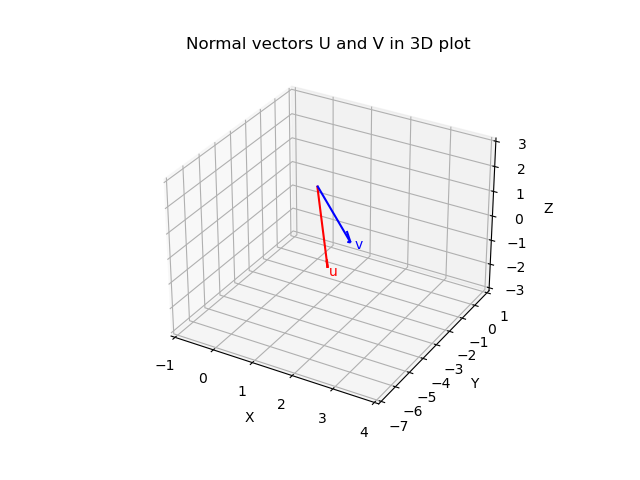
\includegraphics[width=1\linewidth]{figs/plt.png}
\end{frame}

%----------------- C Code -------------------

\begin{frame}[fragile]{C Code (Finding Angle)}
\begin{lstlisting}[language=C]
#include <stdio.h>
#include <math.h>

double find_angle(int A[3], int B[3]) {
    int dot = 0;
    double a_mag = 0;
    double b_mag = 0;
    for (int i=0; i<3; i++) {
        dot += A[i]*B[i];
        a_mag += A[i]*A[i];
        b_mag += B[i]*B[i];
    }

\end{lstlisting}
\end{frame}

\begin{frame}[fragile]{C Code (cont..)}
\begin{lstlisting}[language=C]
    a_mag = pow(a_mag, 0.5);
    b_mag = pow(b_mag, 0.5);
    double cos_theta = dot/(a_mag*b_mag);
    if (cos_theta > 1.0) {
        cos_theta = 1.0; 
    }
    if (cos_theta < -1.0) {
        cos_theta = -1.0;
    }
    return acos(cos_theta);
}
\end{lstlisting}
\end{frame}

%----------------- Python Code -------------------
\begin{frame}[fragile]{Python Code (Calling C)}
\begin{lstlisting}[language=Python]
import ctypes
import numpy

lib = ctypes.CDLL("./computations.so")

lib.find_angle.argtypes = [
    ctypes.POINTER((ctypes.c_int * 3)),
    ctypes.POINTER((ctypes.c_int * 3))
]
lib.find_angle.restype = ctypes.c_double
\end{lstlisting}
\end{frame}


\begin{frame}[fragile]{Python Code (cont..)}
\begin{lstlisting}[language=Python]
def compute_angle(u, v):
    u_arr = (ctypes.c_int * 3)(*u)
    v_arr = (ctypes.c_int * 3)(*v)
    theta = lib.find_angle(u_arr, v_arr)
    return theta

u = [1, -2, -2]
v = [3, -6, 2]
theta = compute_angle(u, v)

print(f"Angle (radians): {theta}")
print(f"Angle (degrees): {theta * 180 / numpy.pi}")
\end{lstlisting}
\end{frame}

\end{document}